\chapter[Heuristics]{Heuristics}

% Introduction
\chapterinitial{I}{t} is often necessary to find the most desirable choice from
a large, or indeed, infinite set of options. Sometimes this can be done using
exact techniques but often this is not possible and finding an almost perfect
choice quickly is just as good. This is where the field of heuristics comes in
to play.

\section{Problem}\label{sec:problem}

A delivery company needs to deliver goods to 13 different stops.
They need to find a route for a driver that stops at each of the stops
once only, then returns to the first stop, the depot.

The stops are drawn in Figure~\ref{fig:tsp}.

\begin{figure}
    \begin{center}
        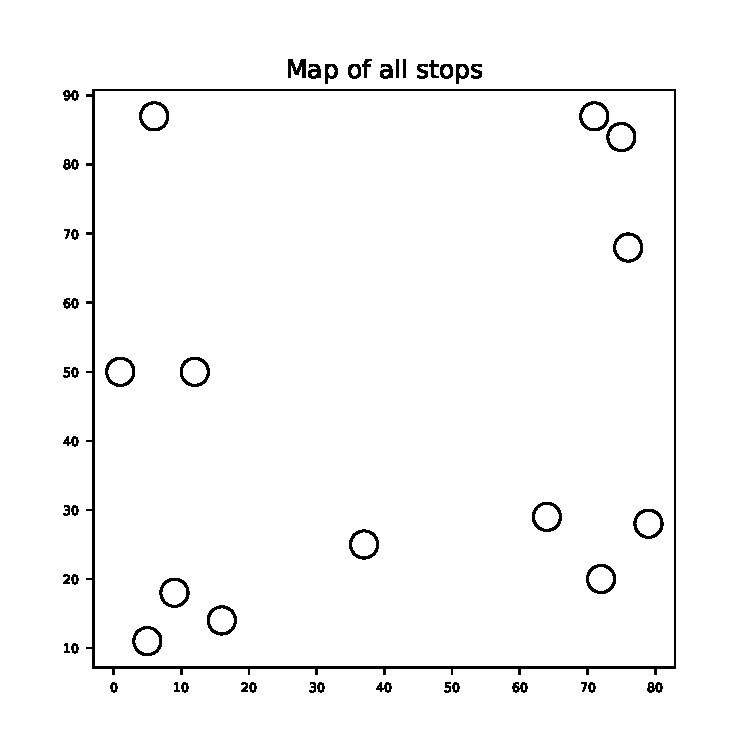
\includegraphics[width=.8\textwidth]{./assets/tsp/main.pdf}
    \end{center}
    \caption{The positions of the required stops.}
    \label{fig:tsp}
\end{figure}

The relevant information is the pairwise distances between each of the stops,
which is given by the distance matrix in equation (\ref{eqn:tsp}).

\tiny{
    \chapter[Modelling with Differential Equations]{Modelling with Differential Equations}

% Introduction
\chapterinitial{S}{ystems} often change in a way that depends on their current
state. For example, the speed at which a cup of coffee cools down depends on its
current temperature. These types of systems are called dynamical systems and are
modelled mathematically using differential equations. In this chapter we will
consider a direct solution approach using symbolic mathematics.

\section{Problem}\label{sec:problem}

Consider the following situation: the entire population of a small rural town
has caught a cold. All 100 individuals will recover at an average rate of 2 per
day.  The town leadership have noticed that being ill costs approximately
\pounds10 per day, this is due to general lack of productivity, poorer mood and
other intangible aspects. They need to decide whether or not to order cold
medicine which would \textbf{double} the recover rate. The cost of of the cold
medicine is a one off cost of \pounds5 per person.
% TODO Find a more realistic example.

\section{Theory}\label{sec:theory}

In the case of this town, the overall rate at which people get better is
dependent on the number of people in how are ill. This can be represented
mathematically using a differential equation which is a way of relating the rate
of change of a system to the state of the system itself.

In general if we are interested in some variable \(x\) over time \(t\) the
differential function equation will be of the form:

\begin{equation}
    \frac{dx}{dt} = f(x)
\end{equation}

For some function \(f\).
In our case,
if we denote the number of infected individuals as \(I\) where we implicitly
mean that \(I\) is a function of time: \(I=I(t)\) and the rate at which
individuals recover by \(\alpha\) then the differential equation
that describes the above situation is:

\begin{equation}
    \frac{dI}{dt} = -\alpha I
\end{equation}

Finding a solution to this differential equation means finding an expression for
\(I\) that when differentiated gives \(- alpha I\).

In this particular case, one such function is:

\begin{equation}
    I(t) = e ^ {-\alpha t}
\end{equation}

However, \(I(0) = 1\) whereas for our problem we know that at time \(t=0\) there
are 100 infected individuals. Indeed a differential equation defines a family of
solutions and we need to know some sort of initial (also referred to as
boundary) condition to have the exact solution. Which in this case would be:

\begin{equation}
    I(t) = 100e ^ {-\alpha t}
\end{equation}

To evaluate the cost we then need to know the sum of the values of that function
over time. Integration gives us exactly this, so the cost would be:

\begin{equation}
    K \int_{0}^{\infty}I(t)dt
\end{equation}

where \(K\) is the cost per person per unit time.

In the upcoming sections we will confirm and use code to carry out the above
efficiently so as to answer the original question.

\section{Solving with Python}\label{sec:solving-with-python}

The first step we will take is to write a function to obtain the differential
equation. Note that here we will be using the Python library
\mintinline{python}{sympy} which allows us to carry out symbolic calculations.

\begin{pyin}
import sympy as sym

t = sym.Symbol("t")
alpha = sym.Symbol("alpha")
I_0 = sym.Symbol("I_0")
I = sym.Function("I")


def get_equation(alpha=alpha):
    """Return the differential equation.

    Args:
        alpha: a float (default: symbolic alpha)

    Returns:
        A symbolic equation
    """
    return sym.Eq(sym.Derivative(I(t), t), -alpha * I(t))
\end{pyin}

Using this we can get the equation that defines the population change over time:

\begin{pyin}
eq = get_equation()
print(eq)
\end{pyin}

which gives:

\begin{pyout}
Eq(Derivative(I(t), t), -alpha*I(t))
\end{pyout}

Note that if you are using Jupyter then your output will actually be a
well rendered mathematical equation:

\[
\frac{d}{d t} I{\left(t \right)} = - \alpha I{\left(t \right)}
\]

Note that we can pass a value to \(\alpha\) if we want to:

\begin{pyin}
eq = get_equation(alpha=1)
print(eq)
\end{pyin}

\begin{pyout}
Eq(Derivative(I(t), t), -I(t))
\end{pyout}

We will now write a function to obtain the solution to this differential

\begin{pyin}
def get_solution(I_0=I_0, alpha=alpha):
    """Return the solution to the differential equation.

    Args:
        I_0: a float (default: symbolic I_0)
        alpha: a float (default: symbolic alpha)

    Returns:
        A symbolic equation
    """
    eq = get_equation(alpha=alpha)
    return sym.dsolve(eq, I(t), ics={I(0): I_0})
\end{pyin}

We can verify the solution discussed previously:

\begin{pyin}
sol = get_solution()
print(sol)
\end{pyin}

which gives:

\begin{pyout}
Eq(I(t), I_0*exp(-alpha*t))
\end{pyout}

\[I(t) = I_0 e ^{-\alpha t}\]

We can use sympy itself to verify the result, by taking the derivative of the
right hand side of our solution.

\begin{pyin}
print(sym.diff(sol.rhs, t) == -alpha * sol.rhs)
\end{pyin}

which gives:

\begin{pyout}
True
\end{pyout}

All of the above has given us the general solution in terms of \(I(0)=I_0\) and
\(\alpha\) however we have written the code in such a way as we can pass the
actual parameters:

\begin{pyin}
sol = get_solution(alpha=2, I_0=100)
print(sol)
\end{pyin}

which gives:

\begin{pyout}
Eq(I(t), 100*exp(-2*t))
\end{pyout}

Now, to calculate the cost we will write a function to integrate our result:

\begin{pyin}
def get_cost(
    I_0=I_0, alpha=alpha, cost_per_person=10, cost_of_cure=0,
):
    """Return the cost.

    Args:
        I_0: a float (default: symbolic I_0)
        alpha: a float (default: symbolic alpha)
        cost_per_person: a float (default: 10)
        cost_of_cure: a float (default: 0)

    Returns:
        A symbolic expression
    """
    I_sol = get_solution(I_0=I_0, alpha=alpha)
    return (
        sym.integrate(I_sol.rhs, (t, 0, sym.oo))
        * cost_per_person
        + cost_of_cure * I_0
    )
\end{pyin}

We can now obtain the cost without purchasing the cure:

\begin{pyin}
I_0 = 100
alpha = 2
cost_without_cure = get_cost(I_0=I_0, alpha=alpha)
print(cost_without_cure)
\end{pyin}

which gives:

\begin{pyout}
500
\end{pyout}


The cost with cure can use the above with a modified \(\alpha\) and a non zero
cost of the cure itself:

\begin{pyin}
cost_of_cure = 5
cost_with_cure = get_cost(
    I_0=I_0, alpha=2 * alpha, cost_of_cure=cost_of_cure
)
print(cost_with_cure)
\end{pyin}

which gives:

\begin{pyout}
750
\end{pyout}

So given the current parameters it is not worth purchasing the cure.

\section{Solving with R}\label{sec:solving-with-R}

R has some capability for symbolic mathematics, however at the time of writing
the options available are somewhat limited and/or not reliable. As such, we will
actually solve the problem with R using a numerical integration approach. For an
outline of the theory behind this approach see Chapter % TODO Add reference to chapter

First we write a function to give us the derivative for a given value of \(I\).

\begin{Rin}
derivative <- function(t, y, parameters) {
  with(as.list(c(y, parameters)), {
    dIdt <- -alpha * I  # nolint
    list(dIdt)  # nolint
  })
}
\end{Rin}

For example, to see the value of the derivative when \(I=0\) we have:

\begin{Rin}
derivative(t = 0, y = c(I = 100), parameters = c(alpha = 2))
\end{Rin}

This gives:

\begin{Rout}
[[1]]
[1] -200

\end{Rout}

We will now make use of the \mintinline{R}{deSolve} library for solving
differential equations numerically:

\begin{Rin}
library(deSolve)  # nolint
integrate_ode <- function(times,
                          y0 = c(I = 100),
                          alpha = 2) {
  params <- c(alpha = alpha)
  ode(y = y0, times = times, func = derivative, parms = params)
}
\end{Rin}

This will return a sequence of time point and values of \(I\) at those time
points. Using this we can compute the cost. Note that this function uses
\mintinline{R}{stopifnot} to make sure our differential equation has been solved
for a long enough time period.

\begin{Rin}
get_cost <- function(
                     I_0 = 100,
                     alpha = 2,
                     cost_per_person = 10,
                     cost_of_cure = 0,
                     step_size = 0.0001,
                     max_time = 10) {
  times <- seq(0, max_time, by = step_size)
  out <- integrate_ode(times,
    y0 = c(I = I_0),
    alpha = alpha
  )
  number_of_observations <- length(out[, "I"])

  stopifnot(out[number_of_observations, "I"] < step_size)

  number_of_daily_infections <- sum(
    diff(out[, "time"]) *
      out[-number_of_observations, "I"]
  )
  number_of_daily_infections *
    cost_per_person + cost_of_cure *
      I_0
}
\end{Rin}

Using this we can compute the costs:

\begin{Rin}
alpha <- 2
cost_without_cure <- get_cost(alpha = alpha)
print(round(cost_without_cure))
\end{Rin}


which gives:

\begin{Rout}
[1] 500
\end{Rout}

The cost with cure can use the above with a modified \(\alpha\) and a non zero
cost of the cure itself:

\begin{Rin}
cost_of_cure <- 5
cost_with_cure <- get_cost(
    alpha = 2 * alpha, cost_of_cure = cost_of_cure
)
print(round(cost_with_cure))
\end{Rin}

which gives:

\begin{Rout}
[1] 750
\end{Rout}

So given the current parameters it is not worth purchasing the cure.

\section{Research}\label{sec:research}

TBA

}
\normalsize

The value \(d_{ij}\) gives the travel distance between
stops \(i\) and \(j\). For example, \(d_{23}=67\) % TODO If the distance matrix changes, this value need to be updated
indicates that the distance between the 2nd and 3rd stop in the route is 67. % TODO If the distance matrix changes, this value need to be updated


The delivery company would like to find the route around the 13 stops that gives
the smallest overall travel distance.


\section{Theory}\label{sec:theory}

This problem is called a travelling salesman problem, which can 
often be inefficient to solve using exact methods.
%TODO add footnote reference
Heuristics are a family of methods that can be used to find a find a
\emph{sufficiently good} solution, though not necessarily the optimal solution,
where the emphasis is on prioritising computational efficiency.

The heuristic approach taken here will be to use a neighbourhood search algorithm.
This algorithm works by considering a given potential solution, evaluating it
and then trying another potential solution \emph{close} to it. What \emph{close}
means depends on different approaches and problems: it is referred to as the
neighbourhood. When a new solution is considered \emph{good} (this is
again a term that depends on the approach and problem) then the search
continues from the neighbourhood of this new solution.

For this problem, the steps are to first represent a possible solution, that is a given route
between all the potential stops as a \emph{tour}. If there are 3 total stops
and require that the tour starts and stops at the first one then there are two
possible tours:

\[
    t \in \{(1, 2, 3, 1), (1, 3, 2, 1)\}
\]

Given a distance matrix \(d\) such that \(d_{ij}\) is the distance between stop
\(i\) and \(j\) the total cost of a tour is given by:

\[
    C(t)=\sum_{i=1}^{n} d_{t_i, t_{i + 1}}
\]

Thus, with:

\[
    d = \begin{pmatrix}
        0 & 1 & 3\\
        1 & 0 & 15\\
        3 & 3 & 7
        \end{pmatrix}
\]

We have:

\begin{eqnarray*}
    C((1, 2, 3, 1)) &= d_{12} + d_{23} + d_{31} = 1 + 15 + 3 = 19\\
    C((1, 3, 2, 1)) &= d_{13} + d_{32} + d_{21} = 3 + 3 + 1 = 7
\end{eqnarray*}

Using this framework, the neighbourhood search can be written down as:

\begin{enumerate}
    \item Start with a given tour: \(t\).
    \item Evaluate \(C(t)\).
    \item Identify a new \(\tilde t\) from \(t\) and accept it as a replacement
        for \(t\) if \(C(\tilde t)< C(t)\).
    \item Repeat the 3rd step until some stopping condition is met.
\end{enumerate}

This is shown diagrammatically in Figure~\ref{fig:tsp}.

\begin{figure}[!hbtp]
    \begin{center}
        \includestandalone[width=.7\textwidth]{./assets/neighbourhood_search_flow_diagram/main}
    \end{center}
    \caption{The general neighbourhood search algorithm. \(N(t)\) refers to some
    neighbourhood of \(t\).}
    \label{fig:tsp}
\end{figure}

A number of stopping conditions can be used including some specific
overall cost or a number of total iterations of the algorithm.

The neighbourhood of a tour \(t\) is taken as some set of tours that can be
obtained from \(t\) using a specific and computationally efficient
\textbf{neighbourhood operator}.

To illustrate two such neighbourhoods operators, consider the following tour on
7 stops:

\[
    t = (0, 1, 2, 3, 4, 5, 6, 0)
\]

One possible neighbourhood is to choose 2 stops at random and swap. For
example, the tour \(\tilde t^{(1)}\in N(t)\) is obtained by swapping the 2rd and 5th
stops.

\[
    \tilde t^{(1)} = (0, 1, 5, 3, 4, 2, 6, 0)
\]

Another possible neighbourhood is to choose 2 stops at random and reversing the
order of all stops between (including) those two stops. For example, the tour
\(\tilde t^{(2)} \in N(t)\) is obtained by reversing the order of all stops between
the 2rd and the 5th stop.

\[
    \tilde t^{(2)} = (0, 1, 5, 4, 3, 2, 6, 0)
\]

Examples of these tours are shown in
Figure~\ref{fig:tsp-effect-of-neighbourhood-operators}.

\begin{figure}[!hbtp]
    \begin{center}
        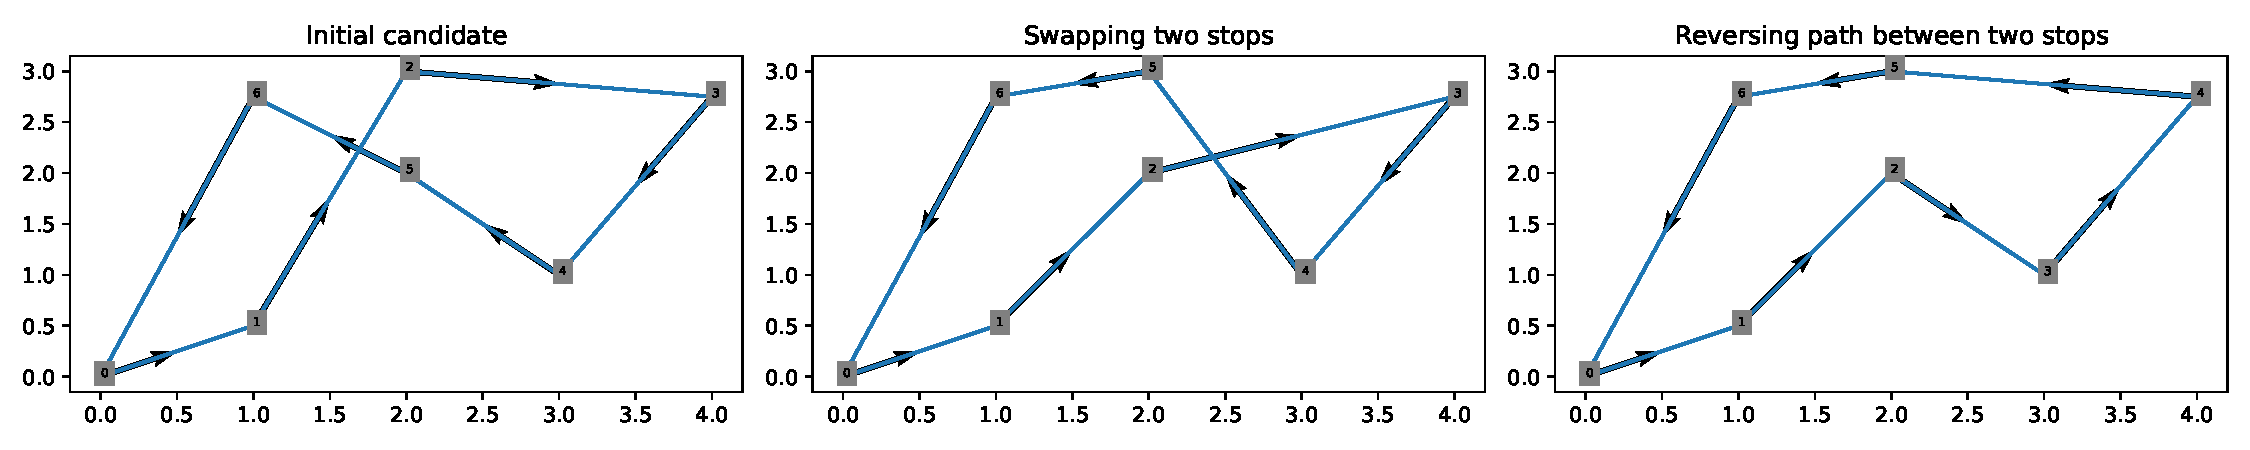
\includegraphics[width=\textwidth]{./assets/tsp-effect-of-neighbourhood-operators/main.pdf}
    \end{center}
    \caption{The effect of two neighbourhood operators on \(t\). \(\tilde t^{(1)}\) is
    obtained by swapping stops 3 and 5. \(\tilde t^{(2)}\) is obtained by reversing the
    path between stops 2 and 5.}
    \label{fig:tsp-effect-of-neighbourhood-operators}
\end{figure}

\section{Solving with Python}\label{sec:solving-with-python}

To solve this problem using Python functions will be written that match the
first three steps in the Section~\ref{sec:theory}.

The first step is to write the \mintinline{python}{get_initial_candidate}
function that creates an initial tour:

\begin{pyin}
import numpy as np


def get_initial_candidate(number_of_stops, seed):
    """Return an random initial tour.

    Args:
        number_of_stops: The number of stops
        seed: An integer seed.

    Returns:
        A tour starting an ending at stop with index 0.
    """
    internal_stops = list(range(1, number_of_stops))
    np.random.seed(seed)
    np.random.shuffle(internal_stops)
    return [0] + internal_stops + [0]
\end{pyin}

This gives a random tour on 13 stops:
% TODO If the number of stops changes this needs to be changed.

\begin{pyin}
number_of_stops = 13
seed = 0
initial_candidate = get_initial_candidate(
    number_of_stops=number_of_stops,
    seed=seed,
)
print(initial_candidate)
\end{pyin}

\begin{pyout}
[0, 7, 12, 5, 11, 3, 9, 2, 8, 10, 4, 1, 6, 0]
\end{pyout}

To be able to evaluate any given tour its cost must be found. Here
\mintinline{python}{get_cost} does this:

\begin{pyin}
def get_cost(tour, distance_matrix):
    """Return the cost of a tour.

    Args:
        tour: A given tuple of successive stops.
        distance_matrix: The distance matrix of the problem.

    Returns:
        The cost
    """
    return sum(
        distance_matrix[current_stop, next_stop]
        for current_stop, next_stop in zip(tour[:-1], tour[1:])
    )
\end{pyin}

\begin{pyin}
distance_matrix = np.array(
    (
        (0, 35, 35, 29, 70, 35, 42, 27, 24, 44, 58, 71, 69),
        (35, 0, 67, 32, 72, 40, 71, 56, 36, 11, 66, 70, 37),
        (35, 67, 0, 63, 64, 68, 11, 12, 56, 77, 48, 67, 94),
        (29, 32, 63, 0, 93, 8, 71, 56, 8, 33, 84, 93, 69),
        (70, 72, 64, 93, 0, 101, 56, 56, 92, 81, 16, 5, 69),
        (35, 40, 68, 8, 101, 0, 76, 62, 11, 39, 91, 101, 76),
        (42, 71, 11, 71, 56, 76, 0, 15, 65, 81, 40, 60, 94),
        (27, 56, 12, 56, 56, 62, 15, 0, 50, 66, 41, 58, 82),
        (24, 36, 56, 8, 92, 11, 65, 50, 0, 39, 81, 91, 74),
        (44, 11, 77, 33, 81, 39, 81, 66, 39, 0, 77, 79, 37),
        (58, 66, 48, 84, 16, 91, 40, 41, 81, 77, 0, 20, 73),
        (71, 70, 67, 93, 5, 101, 60, 58, 91, 79, 20, 0, 65),
        (69, 37, 94, 69, 69, 76, 94, 82, 74, 37, 73, 65, 0),
    )
)
cost = get_cost(
    tour=initial_candidate,
    distance_matrix=distance_matrix,
)
print(cost)
\end{pyin}

\begin{pyout}
827
\end{pyout}

Now a function for neighbourhood operator will be written,
\mintinline{python}{swap_stops}, that swaps two stops in a given tour.

\begin{pyin}
def swap_stops(tour):
    """Return a new tour by swapping two stops.

    Args:
        tour: A given tuple of successive stops.

    Returns:
        A tour
    """
    number_of_stops = len(tour) - 1
    i, j = sorted(
        np.random.choice(range(1, number_of_stops), 2)
    )
    new_tour = list(tour)
    new_tour[i], new_tour[j] = tour[j], tour[i]
    return new_tour
\end{pyin}

Applying this neighbourhood operator to the initial candidate gives:

\begin{pyin}
print(swap_stops(initial_candidate))
\end{pyin}

which swaps the 10th and 12th stops:

\begin{pyout}
[0, 7, 12, 5, 11, 3, 9, 2, 8, 1, 4, 10, 6, 0]
\end{pyout}

Now all the tools are in place to build a tool to carry out the
neighbourhood search \mintinline{python}{run_neighbourhood_search}.

\begin{pyin}
def run_neighbourhood_search(
    distance_matrix,
    iterations,
    seed,
    neighbourhood_operator=swap_stops,
):
    """Returns a tour by carrying out a neighbourhood search.

    Args:
        distance_matrix: the distance matrix
        iterations: the number of iterations for which to
                    run the algorithm
        seed: a random seed
        neighbourhood_operator: the neighbourhood operator
                                (default: swap_stops)

    Returns:
        A tour
    """
    number_of_stops = len(distance_matrix)
    candidate = get_initial_candidate(
        number_of_stops=number_of_stops,
        seed=seed,
    )

    best_cost = get_cost(
        tour=candidate,
        distance_matrix=distance_matrix,
    )

    for _ in range(iterations):
        new_candidate = neighbourhood_operator(candidate)
        if (
            cost := get_cost(
                tour=new_candidate,
                distance_matrix=distance_matrix,
            )
        ) <= best_cost:
            best_cost = cost
            candidate = new_candidate

    return candidate
\end{pyin}

Now running this for 1000 iterations:

\begin{pyin}
number_of_iterations = 1000

solution_with_swap_stops = run_neighbourhood_search(
    distance_matrix=distance_matrix,
    iterations=number_of_iterations,
    seed=seed,
    neighbourhood_operator=swap_stops,
)
print(solution_with_swap_stops)
\end{pyin}

gives:

\begin{pyout}
[0, 7, 2, 8, 5, 3, 1, 9, 12, 11, 4, 10, 6, 0]
\end{pyout}

This has a cost:

\begin{pyin}
cost = get_cost(
    tour=solution_with_swap_stops,
    distance_matrix=distance_matrix,
)
print(cost)
\end{pyin}

\begin{pyout}
362
\end{pyout}

Therefore, using this particular algorithm, a pretty good route is found, with a
total distance of 362.

It is important to note that this may not be the optimal route, and different algorithms
may produce better solutions.
For example, one way to modify the algorithm is to use a different neighbourhood operator.
Instead of swapping two stops, reverse the path between those two
stops. The \mintinline{python}{reverse_path} function does this:

\begin{pyin}
def reverse_path(tour):
    """Return a new tour by reversing the path between two
    stops.

    Args:
        tour: A given tuple of successive stops.

    Returns:
        A tour
    """
    number_of_stops = len(tour) - 1
    i, j = sorted(
        np.random.choice(range(1, number_of_stops), 2)
    )
    new_tour = tour[:i] + tour[i : j + 1][::-1] + tour[j + 1 :]
    return new_tour
\end{pyin}

Applying this neighbourhood operator to the initial candidate gives:

\begin{pyin}
print(reverse_path(initial_candidate))
\end{pyin}

which reverses the order between the 3rd and the 11th stop:

\begin{pyout}
[0, 7, 4, 10, 8, 2, 9, 3, 11, 5, 12, 1, 6, 0]
\end{pyout}

Now running the neighbourhood search for 1000 iterations using the
\mintinline{python}{reverse_path} neighbourhood operator, which corresponds to
an algorithm called the ``2 opt'' algorithm: %TODO add footnote reference

\begin{pyin}
solution_with_reverse_path = run_neighbourhood_search(
    distance_matrix=distance_matrix,
    iterations=number_of_iterations,
    seed=seed,
    neighbourhood_operator=reverse_path,
)
print(solution_with_reverse_path)
\end{pyin}

gives:

\begin{pyout}
[0, 8, 5, 3, 1, 9, 12, 11, 4, 10, 6, 2, 7, 0]
\end{pyout}

This now gives a different route.
Importantly, the costs differ substantially:

\begin{pyin}
cost = get_cost(
    tour=solution_with_reverse_path,
    distance_matrix=distance_matrix,
)
print(cost)
\end{pyin}

which gives:

\begin{pyout}
299
\end{pyout}

This improves on the solution found using the \mintinline{python}{swap_stops}
operator. Figure~\ref{fig:final-tsp-tours-python} shows the final obtained
routes given by both approaches.

\begin{figure}
    \begin{center}
        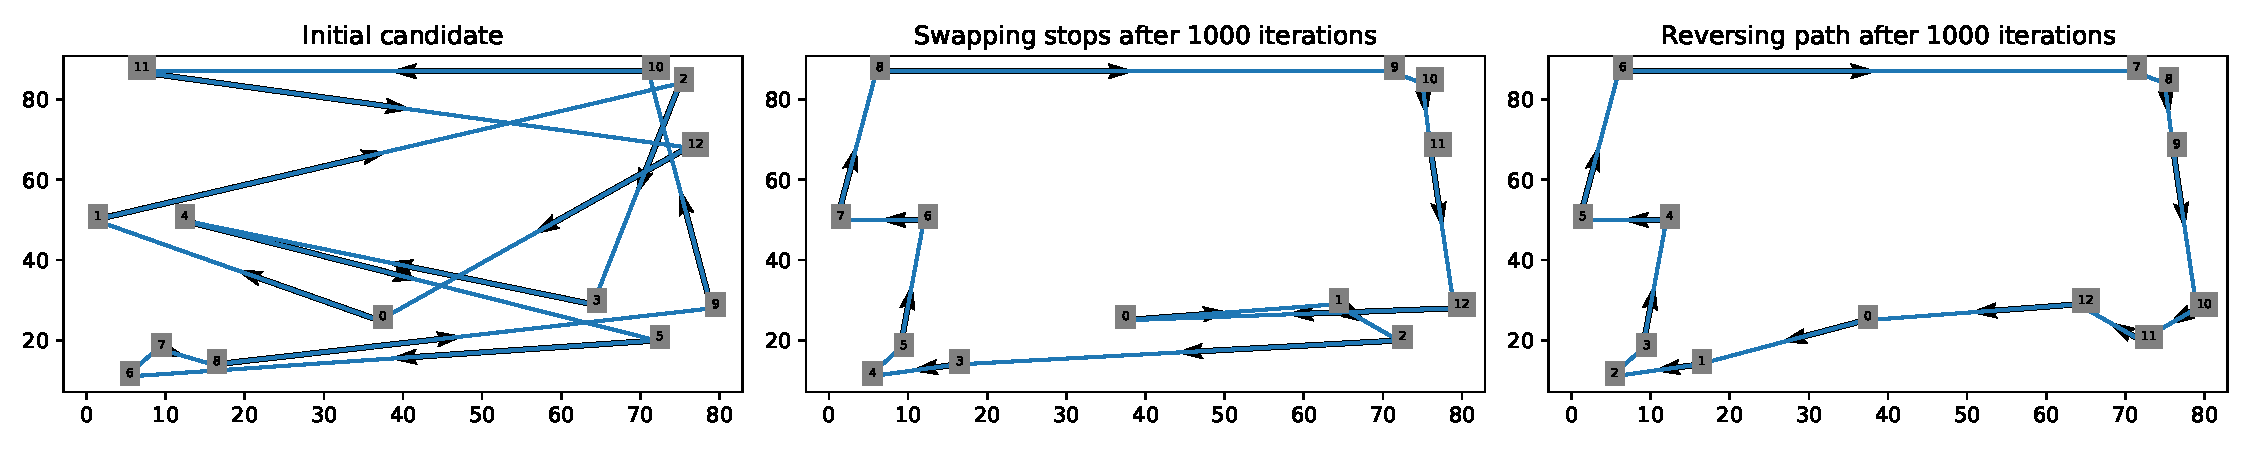
\includegraphics[width=\textwidth]{./assets/final-tsp-tours-with-python/main.pdf}
    \end{center}
    \caption{The final tours obtained by using the neighbourhood search in
    Python.}
    \label{fig:final-tsp-tours-python}
\end{figure}
% TODO Can these plots be squares? to correspond easier with the initial plot of the stop locations. Same with R below.



\section{Solving with R}\label{sec:solving-with-R}

To solve this problem using R, functions will be written that match the
first three steps in the Section~\ref{sec:theory}.

The first step is to write the \mintinline{R}{get_initial_candidate}
function that creates an initial tour:

\begin{Rin}
#' Return an random initial tour.
#'
#' @param number_of_stops The number of stops.
#' @param seed An integer seed.
#'
#' @return A tour starting an ending at stop with index 0.
get_initial_candidate <- function(number_of_stops, seed){
    internal_stops <- 1:(number_of_stops - 1)
    set.seed(seed)
    internal_stops <- sample(internal_stops)
    c(0, internal_stops, 0)
}
\end{Rin}

This gives a random tour on 13 stops:

\begin{Rin}
number_of_stops <- 13
seed <- 1
initial_candidate <- get_initial_candidate(
    number_of_stops = number_of_stops,
    seed = seed)
print(initial_candidate)
\end{Rin}

\begin{Rout}
 [1]  0  9  4  7  1  2  5  3  8  6 11 12 10  0
\end{Rout}

To be able to evaluate any given tour its cost must be found. Here
\mintinline{R}{get_cost}  does this:

\begin{Rin}
#' Return the cost of a tour
#'
#' @param tour A given vector of successive stops.
#' @param seed The distance matrix of the problem.
#'
#' @return The cost
get_cost <- function(tour, distance_matrix){
    pairs <-  cbind(tour[-length(tour)], tour[-1]) + 1
    sum(distance_matrix[pairs])
}
\end{Rin}

\begin{Rin}
distance_matrix <- rbind(
        c(0, 35, 35, 29, 70, 35, 42, 27, 24, 44, 58, 71, 69),
        c(35, 0, 67, 32, 72, 40, 71, 56, 36, 11, 66, 70, 37),
        c(35, 67, 0, 63, 64, 68, 11, 12, 56, 77, 48, 67, 94),
        c(29, 32, 63, 0, 93, 8, 71, 56, 8, 33, 84, 93, 69),
        c(70, 72, 64, 93, 0, 101, 56, 56, 92, 81, 16, 5, 69),
        c(35, 40, 68, 8, 101, 0, 76, 62, 11, 39, 91, 101, 76),
        c(42, 71, 11, 71, 56, 76, 0, 15, 65, 81, 40, 60, 94),
        c(27, 56, 12, 56, 56, 62, 15, 0, 50, 66, 41, 58, 82),
        c(24, 36, 56, 8, 92, 11, 65, 50, 0, 39, 81, 91, 74),
        c(44, 11, 77, 33, 81, 39, 81, 66, 39, 0, 77, 79, 37),
        c(58, 66, 48, 84, 16, 91, 40, 41, 81, 77, 0, 20, 73),
        c(71, 70, 67, 93, 5, 101, 60, 58, 91, 79, 20, 0, 65),
        c(69, 37, 94, 69, 69, 76, 94, 82, 74, 37, 73, 65, 0)
)
cost <- get_cost(
    tour = initial_candidate,
    distance_matrix = distance_matrix)
print(cost)
\end{Rin}

\begin{Rout}
[1] 709
\end{Rout}

Now a function for a neighbourhood operator will be written,
\mintinline{R}{swap_stops}: swapping two stops in a given tour.

\begin{Rin}
#' Return a new tour by swapping two stops.
#'
#' @param tour A given vector of successive stops.
#'
#' @return A tour
swap_stops <- function(tour){
    number_of_stops <- length(tour) - 1
    stops_to_swap <- sort(sample(2:number_of_stops, 2))
    new_tour <- replace(x = tour,
                        list = stops_to_swap,
                        values = rev(tour[stops_to_swap]))
    }
\end{Rin}

Applying this neighbourhood operator to the initial candidate gives:

\begin{Rin}
print(swap_stops(initial_candidate))
\end{Rin}

which swaps the 6th and 11th stops:

\begin{Rout}
 [1]  0  9  4  7  1 11  5  3  8  6  2 12 10  0
\end{Rout}

Now we have all the tools in place to build a tool to carry out the
neighbourhood search \mintinline{R}{run_neighbourhood_search}.

\begin{Rin}
#' Returns a tour by carrying out a neighbourhood search
#'
#' @param distance_matrix: the distance matrix
#' @param iterations: the number of iterations for
#'                    which to run the algorithm
#' @param seed: a random seed (default: None)
#' @param neighbourhood_operator: the neighbourhood operation
#'                                (default: swap_stops)
#'
#' @return A tour
run_neighbourhood_search <- function(
  distance_matrix,
  iterations,
  seed = NA,
  neighbourhood_operator = swap_stops
){
  number_of_stops <- nrow(distance_matrix)
  candidate <- get_initial_candidate(
    number_of_stops = number_of_stops,
    seed = seed
    )

  best_cost <- get_cost(
    tour = candidate,
    distance_matrix = distance_matrix
    )

  for (repetition in 1:iterations) {
    new_candidate <- neighbourhood_operator(candidate)
    cost <- get_cost(
        tour = new_candidate,
        distance_matrix = distance_matrix)

    if (cost <= best_cost) {
      best_cost <- cost
      candidate <- new_candidate
    }

  }
  candidate
}
\end{Rin}

Now running this for 1000 iterations:

\begin{Rin}
number_of_iterations <- 1000
solution_with_swap_stops <- run_neighbourhood_search(
    distance_matrix = distance_matrix,
    iterations = number_of_iterations,
    seed = seed,
    neighbourhood_operator = swap_stops
)
print(solution_with_swap_stops)
\end{Rin}

gives:

\begin{Rout}
 [1]  0 11  4 10  6  2  7 12  9  1  3  5  8  0
\end{Rout}

This has a cost:

\begin{Rin}
cost <- get_cost(
    tour = solution_with_swap_stops,
    distance_matrix = distance_matrix
)
print(cost)
\end{Rin}

which gives:

\begin{Rout}
[1] 360
\end{Rout}

Therefore, using this particular algorithm, a pretty good route is found, with a
total distance of 373.

It is important to note that this may not be the optimal route, and different algorithms
 may produce better solutions.
For example, one way to modify the algorithm is to use a different neighbourhood operator.
Instead of swapping two stops, reverse the path between those two
stops. The \mintinline{R}{reverse_path} function does this:


\begin{Rin}
#' Return a new tour by reversing the path between two stops.
#'
#' @param tour A given vector of successive stops.
#'
#' @return A tour
reverse_path <- function(tour){
    number_of_stops <- length(tour) - 1
    stops_to_swap <- sort(sample(2:number_of_stops, 2))
    i <- stops_to_swap[1]
    j <- stops_to_swap[2]
    new_order <- c(
            c(1: (i - 1)),
            c(j:i),
            c( (j + 1): length(tour))
            )
    tour[new_order]
    }
\end{Rin}

Applying this neighbourhood operator to the initial candidate gives:

\begin{Rin}
print(reverse_path(initial_candidate))
\end{Rin}

which reverses the order
between the 3rd and the 13th stop:

\begin{Rout}
 [1]  0  9 10 12 11  6  8  3  5  2  1  7  4  0
\end{Rout}

Now running the neighbourhood search for 1000 iterations using the
\mintinline{R}{reverse_path} neighbourhood operator, which corresponds to
an algorithm called the ``2 opt'' algorithm: %TODO add footnote reference

\begin{Rin}
number_of_iterations <- 1000
solution_with_reverse_path <- run_neighbourhood_search(
    distance_matrix = distance_matrix,
    iterations = number_of_iterations,
    seed = seed,
    neighbourhood_operator = reverse_path
)
print(solution_with_reverse_path)
\end{Rin}

gives:

\begin{Rout}
 [1]  0  7  2  6 10  4 11 12  9  1  3  5  8  0
\end{Rout}

This now gives a different route.
Importantly, the costs differ substantially:

\begin{Rin}
cost <- get_cost(
    tour = solution_with_reverse_path,
    distance_matrix = distance_matrix
)
print(cost)
\end{Rin}

which gives:

\begin{Rout}
[1] 299
\end{Rout}

This is an improvement on the solution found using the \mintinline{R}{swap_stops}
operator. Figure~\ref{fig:final-tsp-tours-r} shows the final obtained routes
given by both approaches.


\begin{figure}
    \begin{center}
        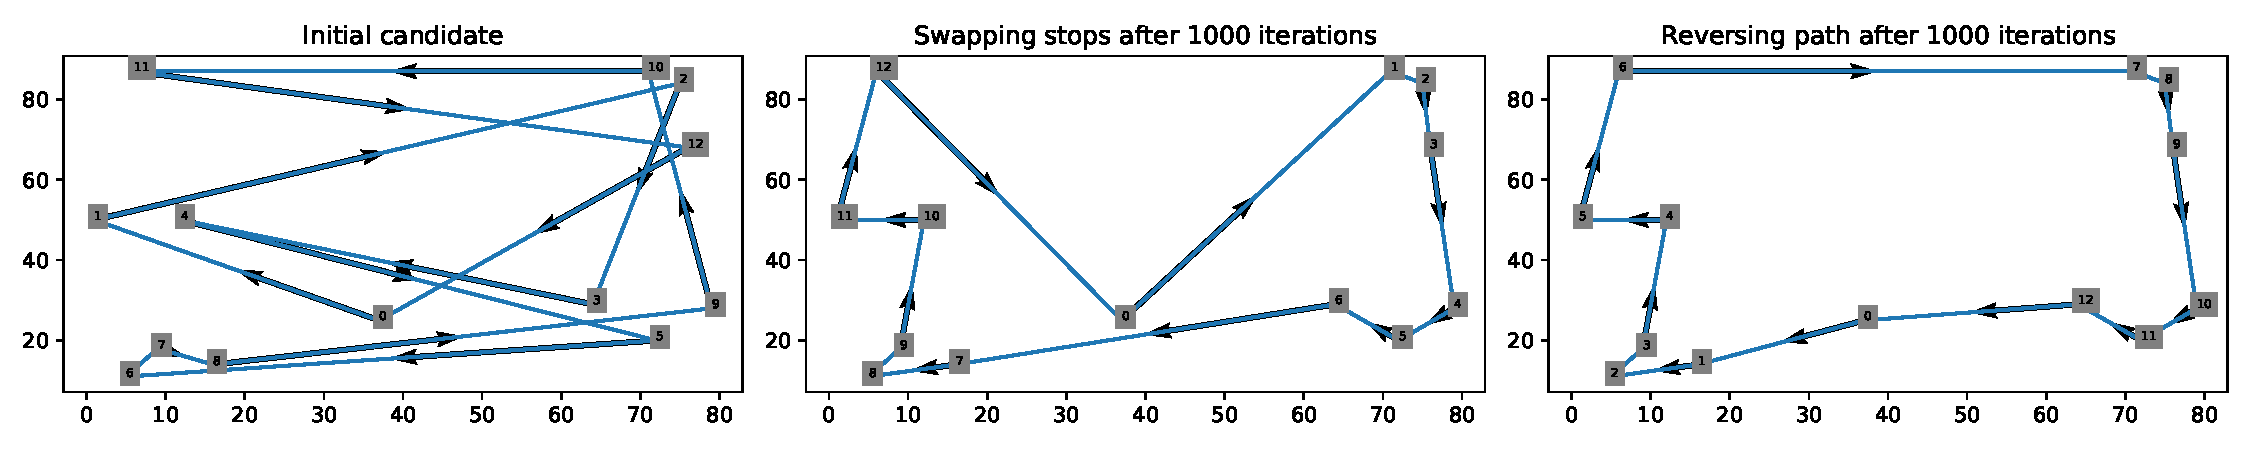
\includegraphics[width=\textwidth]{./assets/final-tsp-tours-with-R/main.pdf}
    \end{center}
    \caption{The final tours obtained by using the neighbourhood search in R}
    \label{fig:final-tsp-tours-r}
\end{figure}

\section{Research}\label{sec:research}

TBA
